\documentclass[main]{subfiles}


\begin{document}
	\begin{lect} {2019-09-23}
		\begin{Reminder}[исправление ошибки-теоремы про длину кривой со стр. 7?]
			\[\abs{\sum \abs{f(t_i) - f(t_{i - 1})}} - \sum \abs{\abs{f(t_i) - f(t_{i - 1} )} -
			\abs{f'(\tau_i)\Delta t_i}} \leq \]
			\[\leq \sum \abs{\int_{t_{i - 1}} ^{t_i} \abs{f'(t)} dt - \int_{t_{i - 1}}^{t_i} \abs{f'(\tau_i)}dt} = \]
			\[\sum \int_{t_{i - 1} }^{t_i} \abs{f'(t) - f'(t_i)}dt < \sum \mathcal{E} \Delta_i t = \mathcal{E}(b - a)\]
			\[\forall \mathcal{E} > 0 \q \exists \delta > 0 \text{ если } f_i - f_{i - 1} < \delta \]
			\[\Ra \abs{f'(t) - f'(\tau_i)} < \mathcal{E}\]
		\end{Reminder}

		\begin{Lemma} \
			\begin{figure}[H]
			    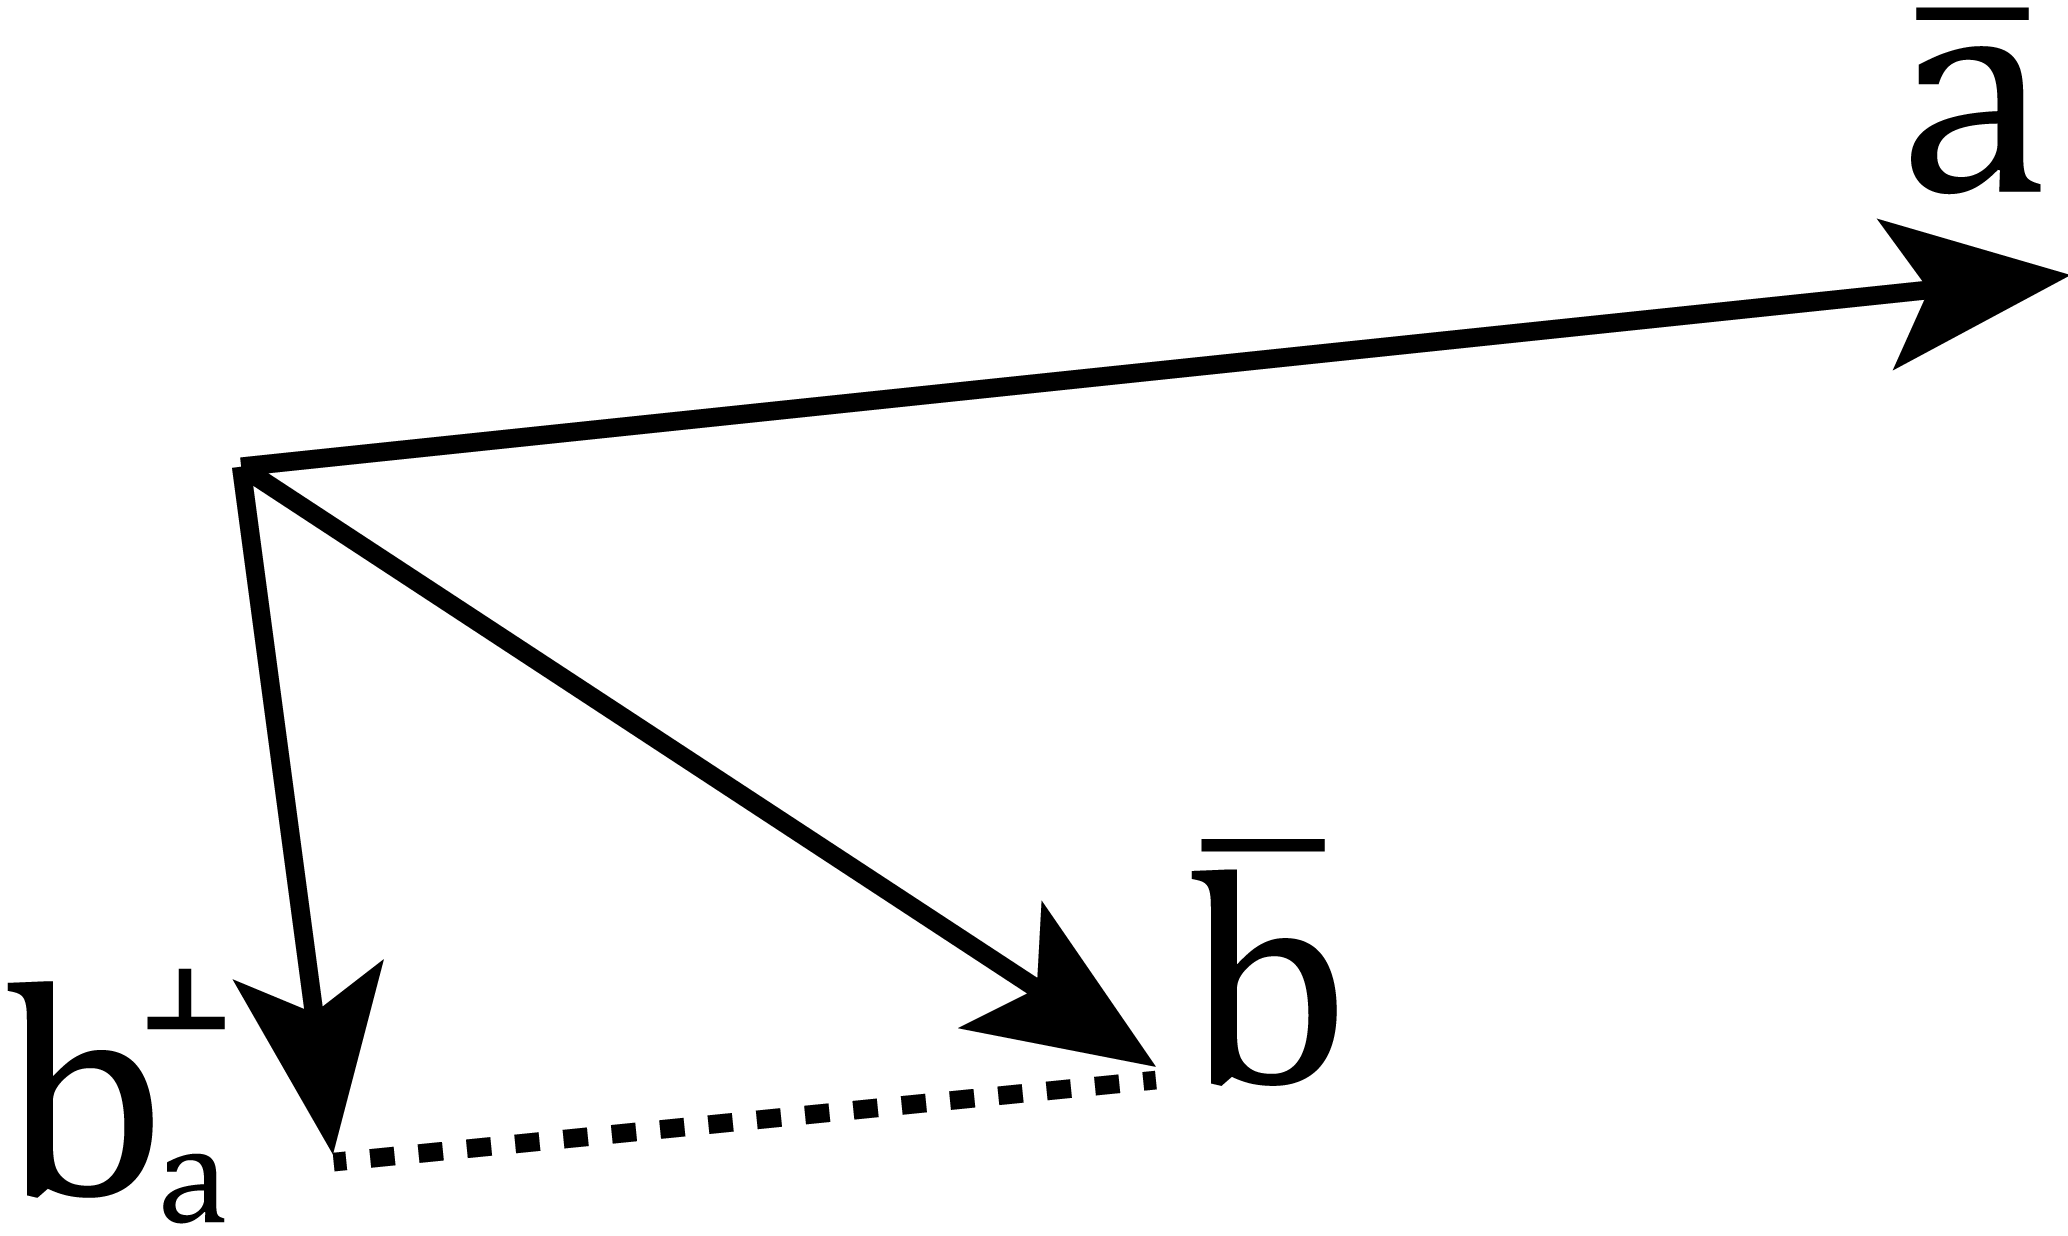
\includegraphics[width=4cm]{pics/3_1.png}
			    \centering
			\end{figure}

				\[\vec{b} = \text{Пр}_a b + b \frac{1}{a}\]
				\[\vec{\text{Пр}_a b} = \frac{(a, b)}{\abs{a}^2} \vec{a}\]
				\[\abs{b \frac{1}{a}} = \frac{\abs{\vec{a} \times \vec{b}}}{\abs{a}}\]
		\end{Lemma}

		\begin{Proof} \
			\begin{figure}[H]
			    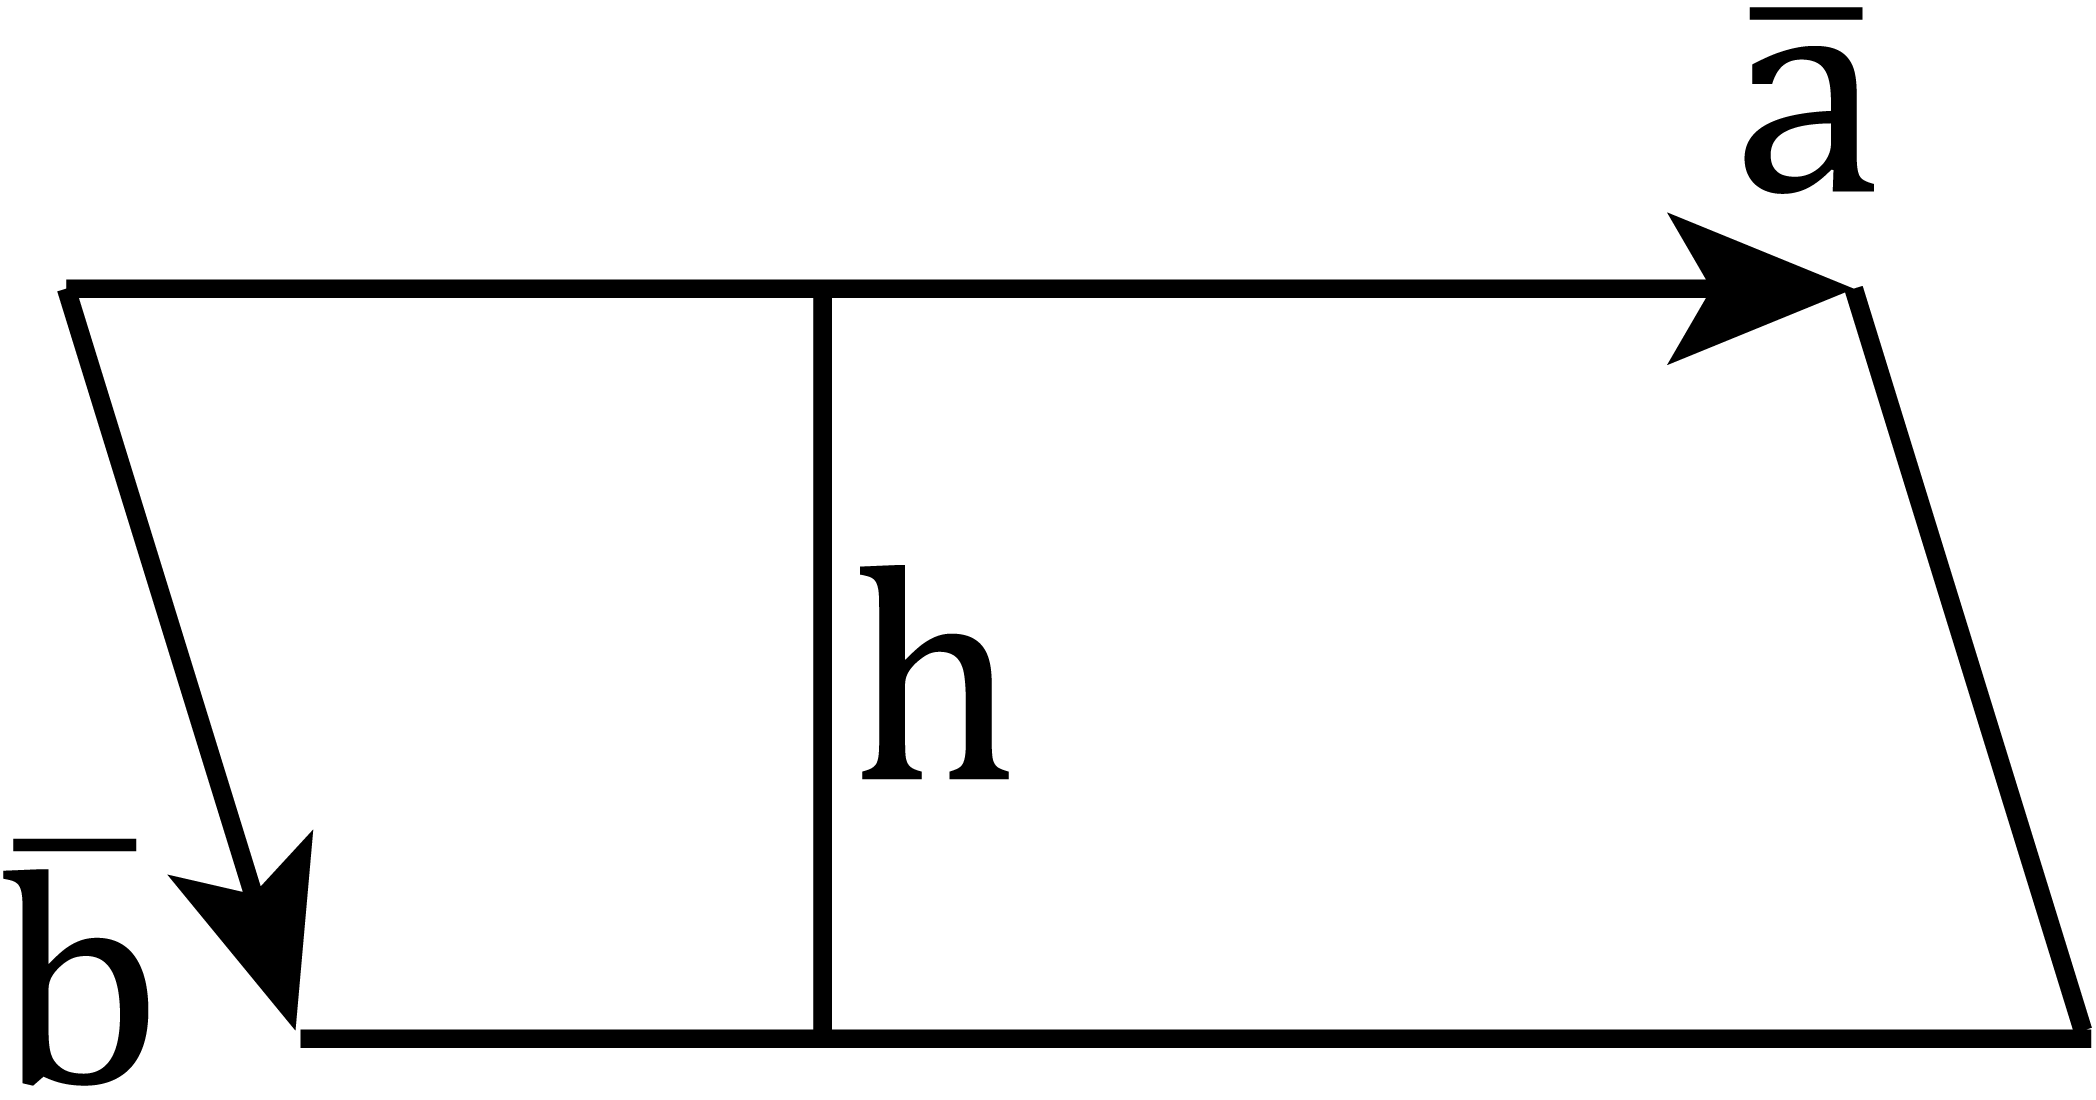
\includegraphics[width=4.5cm]{pics/3_2.png}
			    \centering
			\end{figure}

			\[h = \frac{S}{\abs{a}}\]
			\[\frac{(\vec{a} \times \vec{b}) \times \vec{a}}{\abs{a}^2} = b \frac{1}{a}\]
			\[(a, b, a \times b) \text{ - прав. тройка}\]
			\[(a \times b, a, b) \text{ - прав. тройка}\]
		\end{Proof}

		\begin{Theorem}\
			\begin{figure}[H]
			    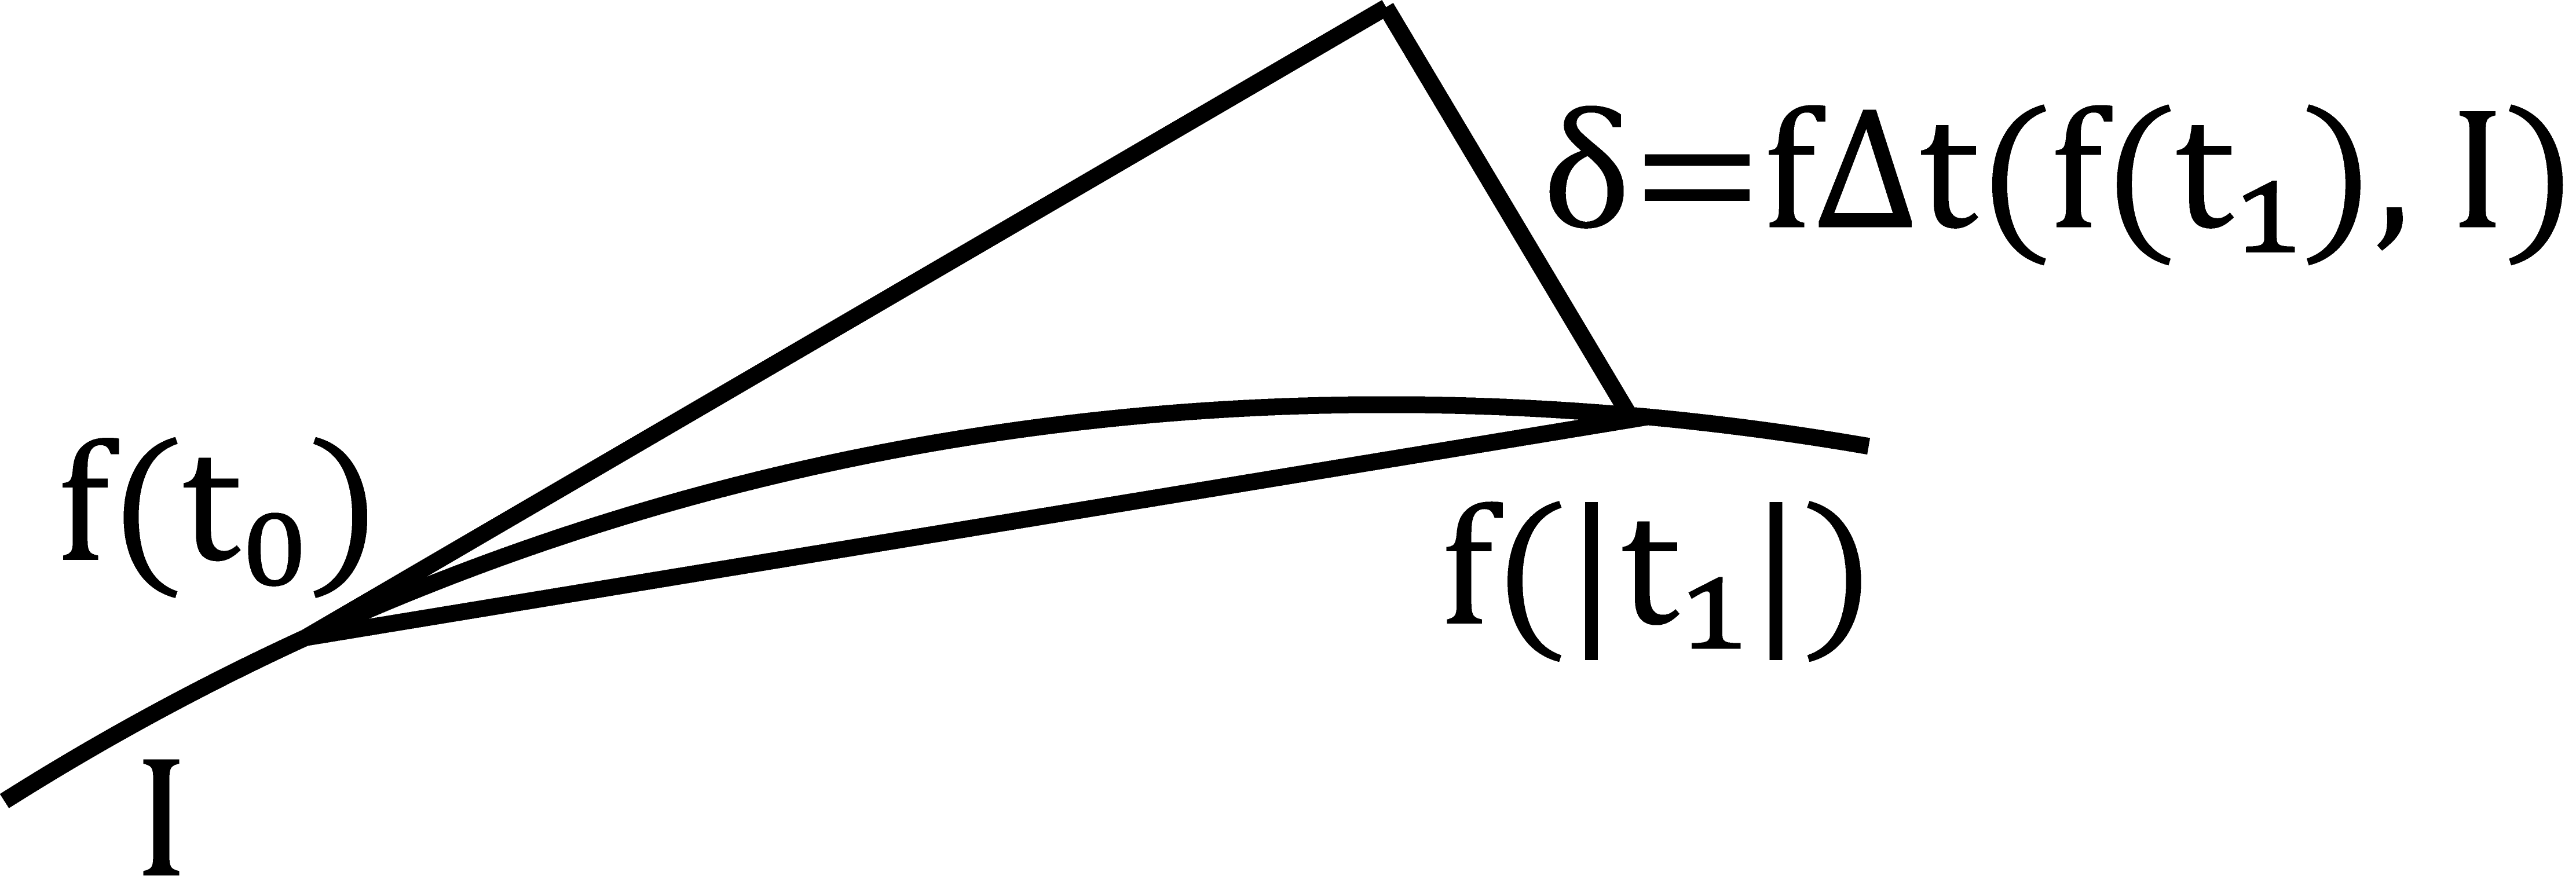
\includegraphics[width=7.5cm]{pics/3_3.png}
			    \centering
			\end{figure}

			\[\lim_{t_1 \to t_0}  \frac{\delta}{\abs{f(t_1) - f(t_0)}} = 0\]
		\end{Theorem}

        \begin{Proof}
            \[\vec{f'}(t_0) \Ra \text{ по лемме}\]
			\[\delta = \frac{\abs{f'(t_0) \times (f(t_1) - f(t_0))}}{\abs{f'(t_0)}}\]
			\[\lim_{t_1 \to t_0} \frac{\delta}{f(t_1) - f(t_0)} =
			\lim_{t_1 \to t_0} \frac{\abs{f'(t_0) \times (f(t_1) - f(t_0))}}{\abs{f'(t_0)} \cdot \abs{f(t_1) - f(t_0)}}\]
			\[\lim_{t_1 \to t_0} \frac{\abs{f'(t_0) \times \frac{f(t_1) - f(t_0)}{t_1 - t_0}}}
			{\abs{f'(t_0) \cdot \abs{\frac{f(t_1) - f(t_0)}{t_1 - t_0}}}} =
			\frac{f'(t_0) \times f'(t_0)}{\abs{f'(t_0)}^2} = 0\]
			$\La \text{очев}$
        \end{Proof}

		\subsection{Вектор кривизны}
		\begin{Definition} \
			\begin{figure}[H]
			    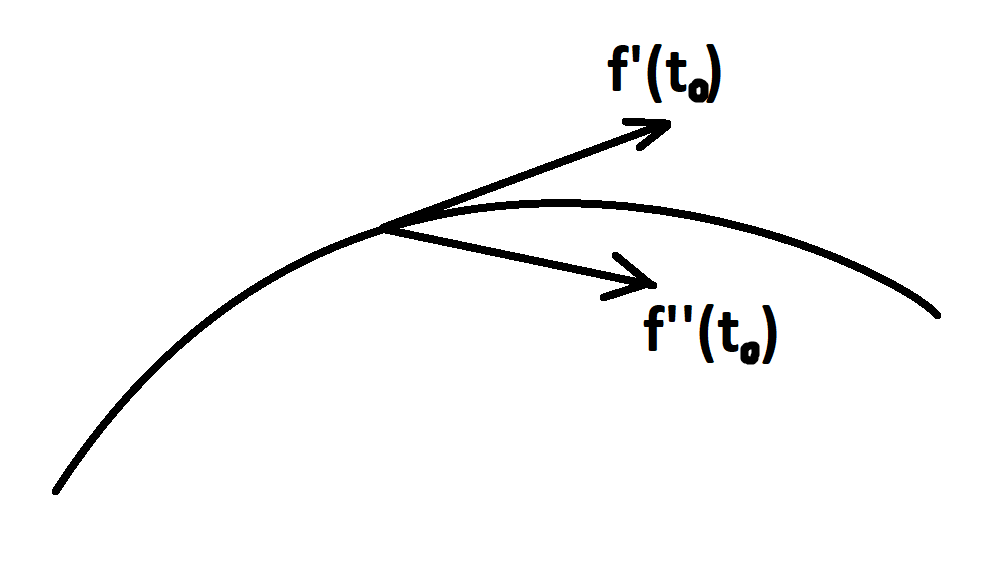
\includegraphics[width=5cm]{pics/3_4.png}
			    \centering
			\end{figure}

			\[g(\varphi(t)) = g(s) = f(t) \q\q s = \varphi(t)\]
			\[\vec{f'}(t) = (g(\varphi_i t_i))' = \vec{g'} \cdot \varphi'(t)\]
			\[\vec{v}(t_0) = \frac{f'(t_0)}{\abs{f'(t_0)}} \q\q \vec{n} : \abs{n} = 1; \q \vec{n} \perp \vec{v}\]
			\[n \in <f', f''> \q \vec{n} \text{ и } \vec{f}'' \text{ в одной полуплоскости } f'(t)\]
			\[\vec{v}'(t) \perp \vec{v}(t)\]
			\[\vec{v}'(t) = k \cdot \vec{n}\]
			\[\abs{n} = 1 \q k(t) \text{ - \underline{кривизна кривой}} \q k(t) \geq 0 \text{ в точке } t\]
			\[\vec{n} \text{ - вектор главной нормали}\]
			\[\vec{v} \text{ - касат. вект}\]
		\end{Definition}

		\begin{Utv}
			\[f(t) \text{ - натуральная парам.}\]
			\[\abs{f'(t)} = 1 \Ra v = f'(t)\]
			\[f''(t) = k \vec{n}\]
			\[\vec{n} = \frac{f''(t)}{\abs{f''(t)}}\]
			\[k = \abs{f''(t)}\]
			%рисунок 5 (центростр. ускорение)
			\begin{figure}[H]
			    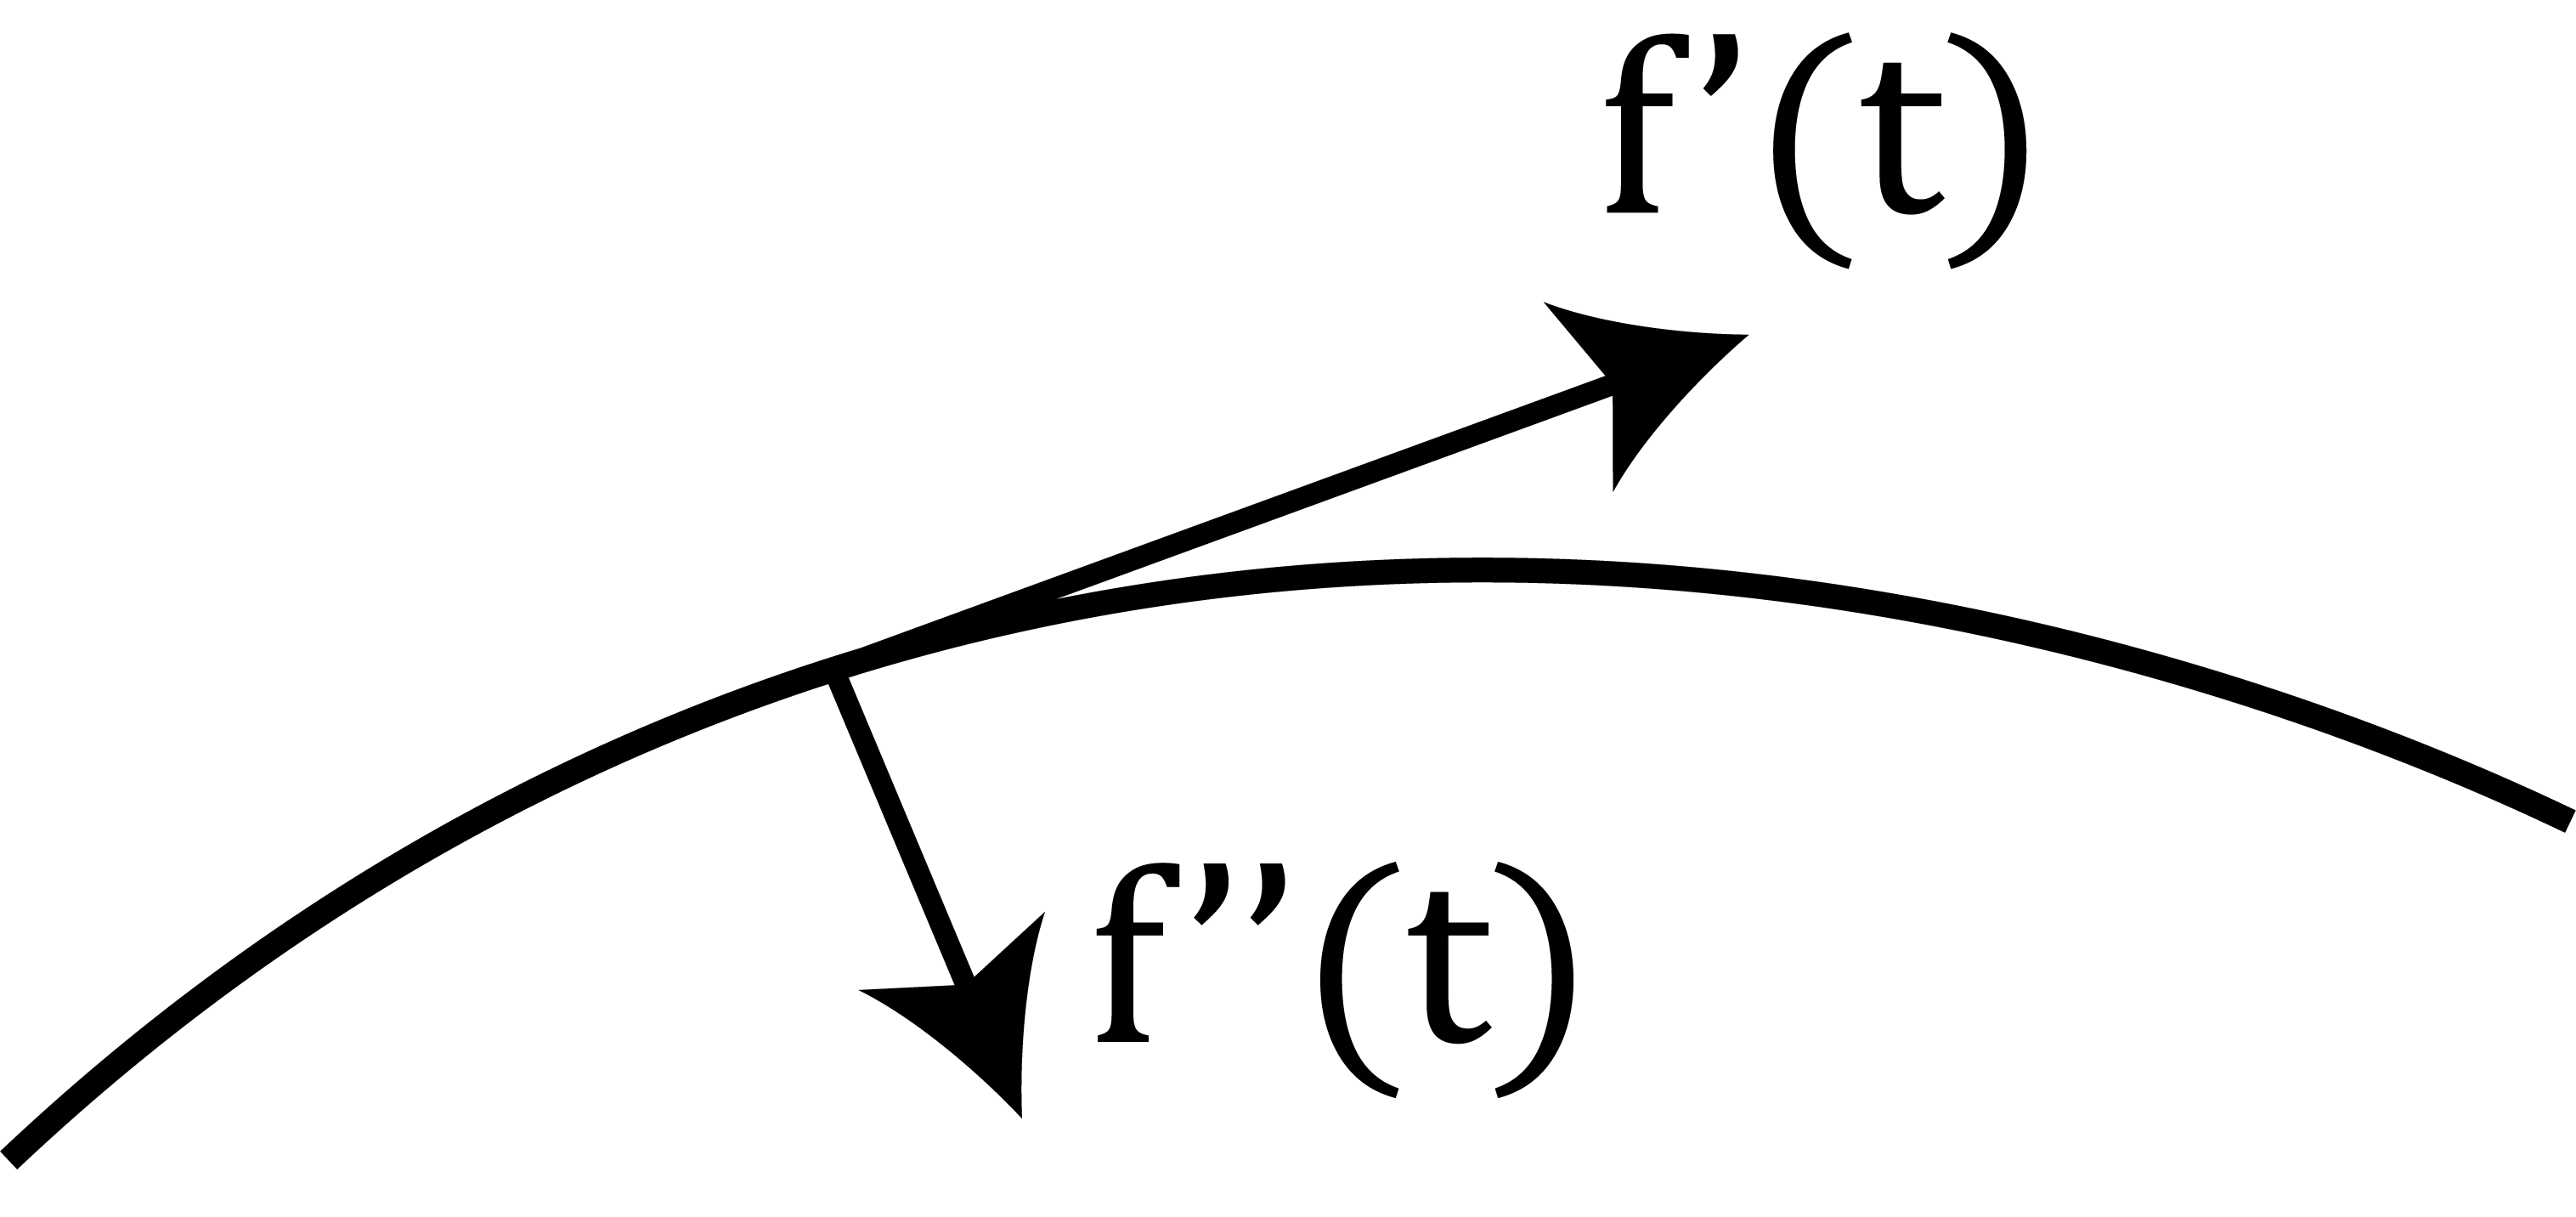
\includegraphics[width=6cm]{pics/3_5.png}
			    \centering
			\end{figure}

			\[f(t) \text{ - любая параметризация, } g(s) \text{ - натур. парам.}\]
			\[f(t) = g(\varphi(t)) \q\q s = \varphi(t) \text{ - нат. парам}\]
			\[s = \underbracket{\int_a^t (f'(\tau)) d\tau}_{ = \varphi(t)} \]
			\[f'(t) = g'(s) \cdot \varphi'(t)\]
			\[f''(t) = (g'(\varphi(t)))' \cdot \varphi'(t) + g'(s) \cdot \varphi''(t) = \]
			\[= \underbracket{g''(s) \cdot \varphi'^2(t)}_{\perp \vec{v}} +
			\underbracket{g'(s) \varphi''(t)}_{ \parallel g'(s) = v}  \]
		\end{Utv}

		\begin{theorem}
			Плоск. на вект $f'(t)$ и $f''(t)$ не зависит от параметризации
		\end{theorem}

		\begin{definition}
			Эта плоскость (на вект. $\vec{v}$ и $\vec{n}$) наз. соприкасающейся плоск.
		\end{definition}

		\subsection{Формула Френе}
		\begin{Definition} \
			\begin{figure}[H]
			    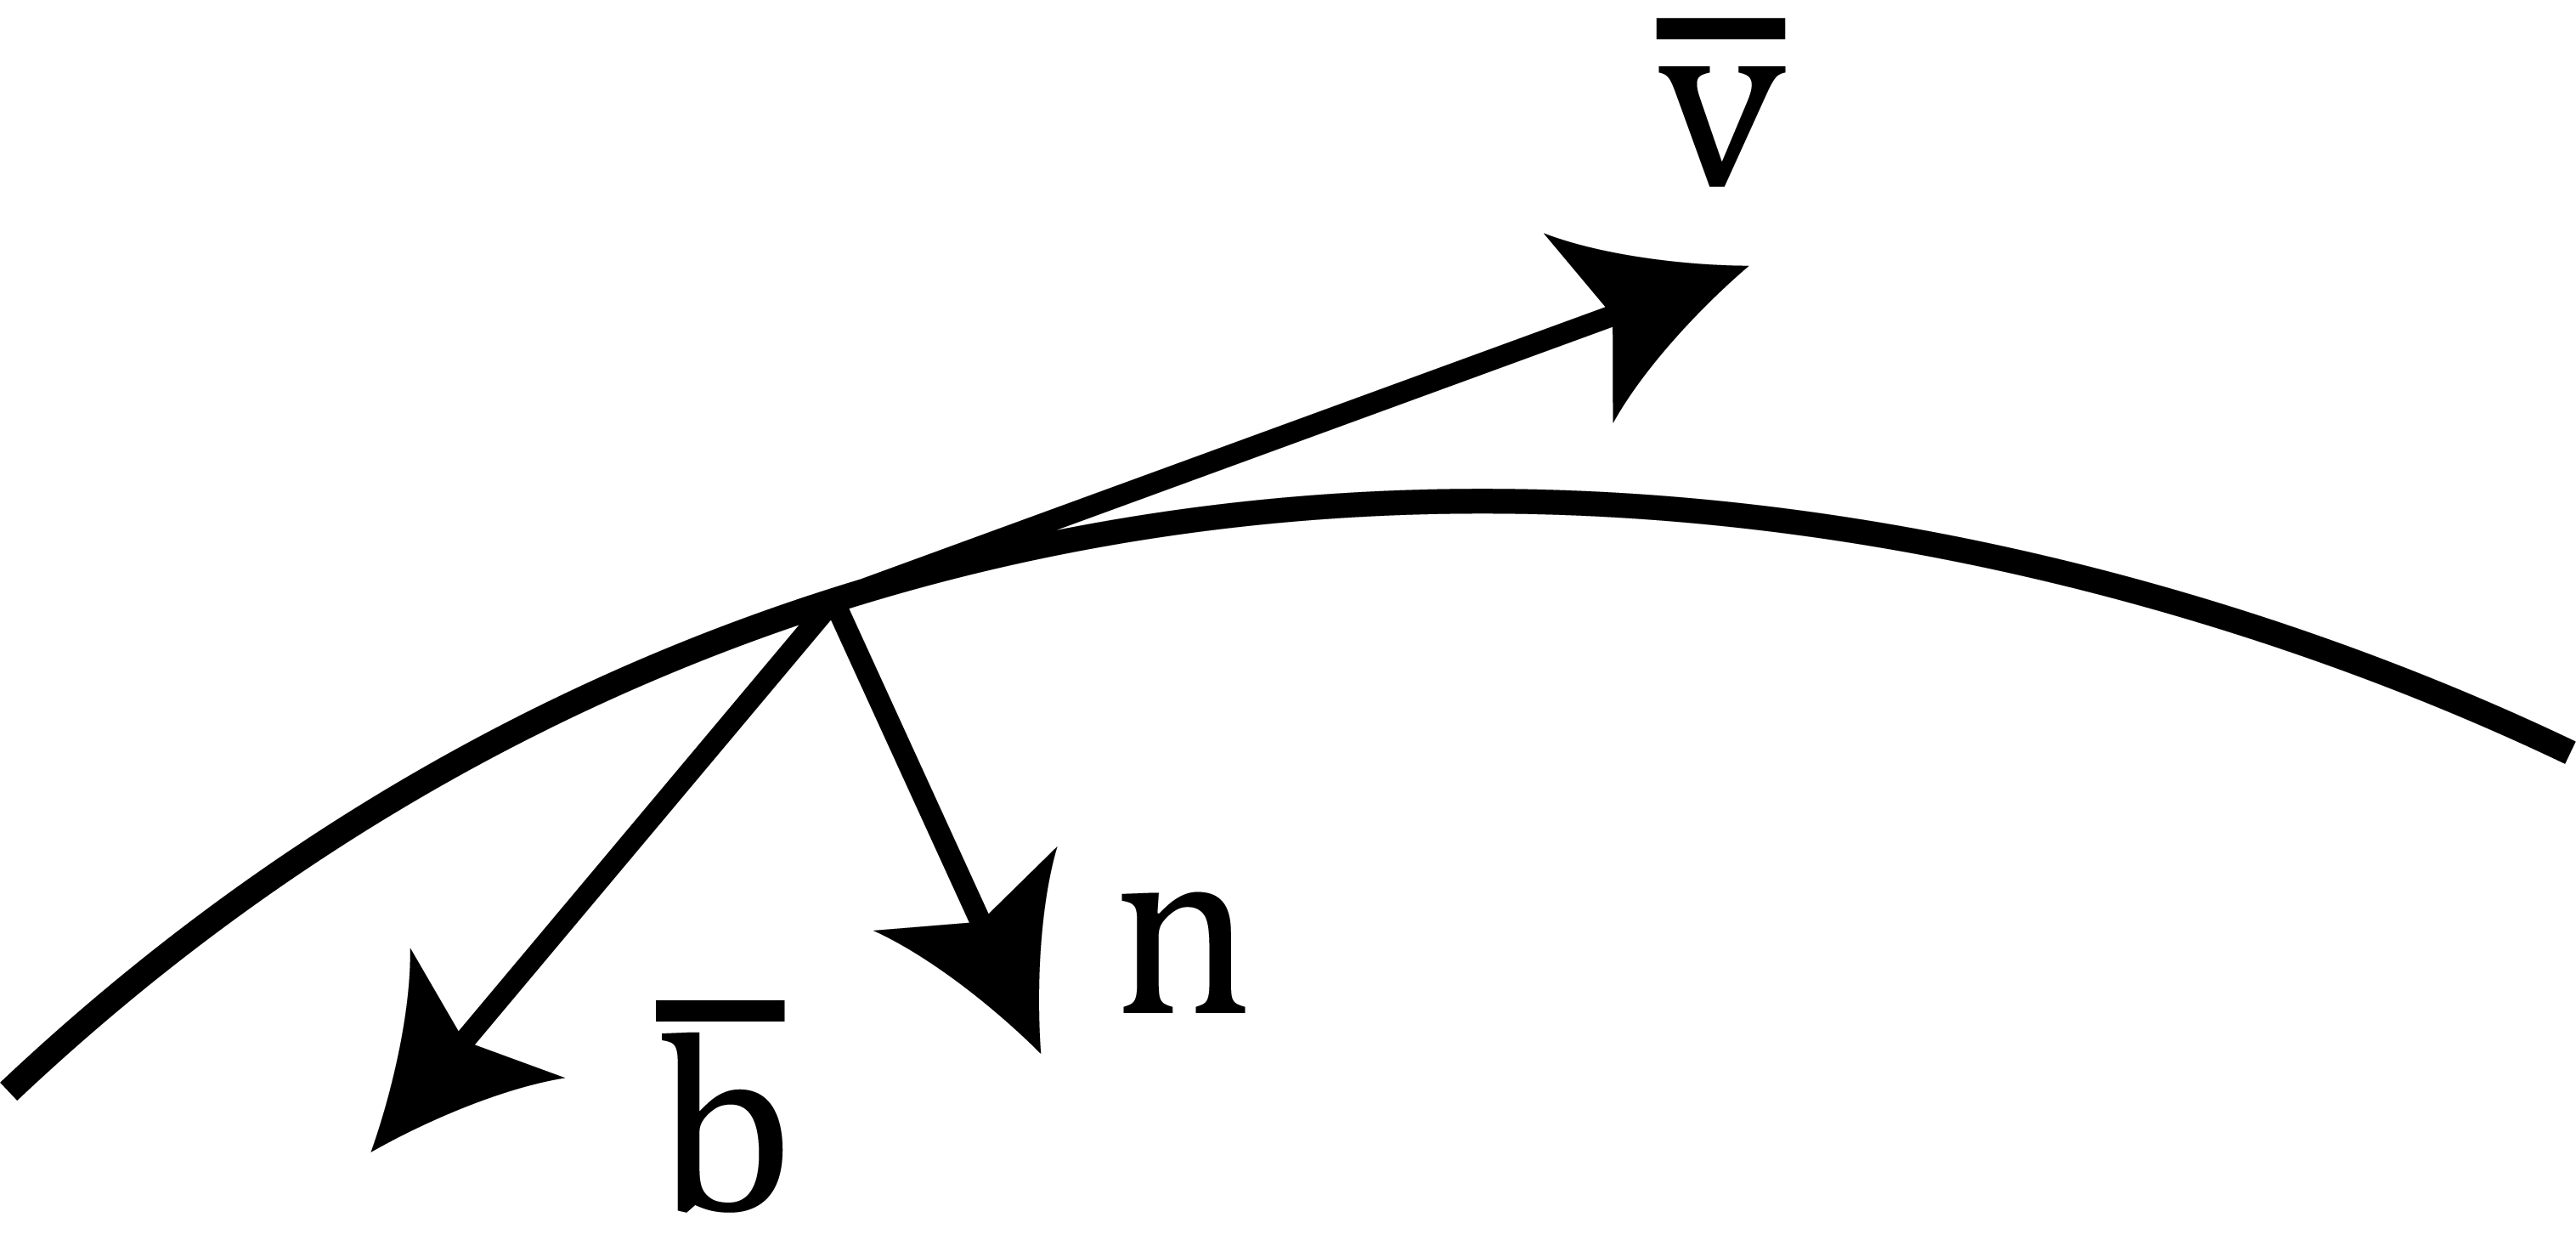
\includegraphics[width=5.5cm]{pics/3_6.png}
			    \centering
			\end{figure}

			\[\vec{b} = \vec{v} \times \vec{n} \text{ - вектор бинормали}\]
			\[(\vec{v}, \vec{n}, \vec{b}) \text{ - базис Френе}\]
			Трехвекторник (трехгранник) Френе или репер Френе
			\[\vec{v}' = k \cdot \vec{n}\]
			\[b' \perp b\]
			\[b' = (\vec{v} \times \vec{n})' = \underbracket{\vec{v}' \times \vec{n}}_{= 0 } +
			\vec{v} \times n' \perp \vec{v}\]
			\[\vec{v}' = k \vec{n}\]
			\[\Ra b' \parallel \vec{n} \Ra b' = -\ae \cdot \vec{n} \text{ - каппа}\]
			\[\ae \text{ называется кручением кривой}\]
		\end{Definition}

		\begin{Theorem}
				\[\ae = 0 \rla \text{ Кривая плоская}\]
				\[\text{Кривая плоская } \rla \text{ она лежит в плоск } <v, n> \rla\]
				\[\rla \text{ нормаль к } <v, n> \text{ постоянна } \rla b = const \rla b' = 0 \rla \ae = 0\]
		\end{Theorem}

		\[n' = (\vec{b} \times v)' = b' \times v + b \times v' = - \ae \  n \times v + k \cdot b \times n = \]
		\[\ae \cdot \vec{b} - k \vec{v}\]
		\[v' = kn\]
		\[n' = -kv + \ae b\]
		\[b' = -\ae n\]
		\[\begin{tabular} {c | c | c | c}
				& v & n & b\\\hline
			 v' & 0 & k & 0\\\hline
			 n' & -k& 0 & \ae\\\hline
			 b' & 0 & -\ae & 0
		\end{tabular}\]

		\subsection{Вычисление кривизны}
		\begin{Theorem}
			\[k = \frac{\abs{f'(t) \times f''(t)}}{\abs{t'(t)}^3}\]
		\end{Theorem}

		\begin{Proof}
			\[g(s) \text{ - нат. парам } f(t) = g(\varphi(t)) \q s = \varphi(t) \q \varphi(t) =
			\int_a^t \abs{f'(\tau)}d\tau\]
			\[g'(s) = \vec{v} \q g''(s) = k\vec{n} \q\q \varphi'(t) = \abs{f'(t)}\]
			\[f''(t) = g''(s) \cdot \varphi^2(t) + g'(s) \cdot \varphi''(t) =
			k \cdot \vec{n} \cdot \abs{f'(t)}^2 + v \cdot \varphi''(t)\]
			\[f''(t) \times f'(t) = k \abs{f'(t)}^2 \cdot \vec{n} \times f'(t) + 0 =  \q\q\q v'(t)
			= \abs{f'(t)}\vec{v}\]
			\[= k \cdot \vec{n} \times \vec{v} \abs{f'(t)}^3\]
			\[\abs{f''(t) \times f'(t)} = k \abs{f'(t)}^3\]
			\[k = \frac{\abs{f''(t) \times f'(t)}}{\abs{f'(t)}^3}\]
		\end{Proof}
	\end{lect}
\end{document}
